\documentclass[conference]{IEEEtran}

% ========= PACKAGES =========
\usepackage{amsmath,amssymb}
\usepackage{graphicx}
\usepackage{tikz}
\usepackage{booktabs}
\usepackage{cite}

% ========= TITLE =========
\title{Magnetic-Laminated On-Chip Microinductor in 0.18 $\mu$m CMOS and Hybrid LDO Application}

\author{
  \IEEEauthorblockN{Shinichi Samizo}
  \IEEEauthorblockA{Independent Researcher\\
  Project Design Hub, Japan\\
  Email: samizo@example.com}
}

\begin{document}
\maketitle

% ========= ABSTRACT =========
\begin{abstract}
This paper proposes a CMOS-compatible magnetic-laminated on-chip microinductor for the 0.18~$\mu$m AMS node. 
By adding a simple post-BEOL magnetic lamination and Patterned Ground Shield (PGS), the limitations of conventional air-core inductors---low $Q$, large area, and insufficient current capacity---are mitigated. 
Applied to a hybrid Buck-LDO regulator, the proposed inductor achieves simultaneous improvements in efficiency, noise, and transient response. 
Target performance around 20~MHz is $L=90$--150~nH, $Q=12$--20, and $I_{\mathrm{sat}}\ge0.5$~A. 
The overall power system reaches $\eta_{\mathrm{total}}\approx 78$--82\%, output ripple $<1$~mV$_{\mathrm{rms}}$, PSRR $>60$~dB@1~MHz, and EMI reduction of 3--6~dB. 
The technique requires only one additional step to the mature CMOS process, enabling rapid application to automotive, IoT, and AMS SoCs.
\end{abstract}

% ========= INTRO =========
\section{Introduction}
The 0.18~$\mu$m AMS CMOS process remains widely used for automotive, industrial, and IoT SoCs thanks to its high-voltage devices (20--60~V LDMOS), high-temperature operation (125--150$^\circ$C), and long-term supply. 
Conventional IVRs rely on external inductors, which suffer from increased BOM, reduced reliability, and EMI issues. 
Air-core on-chip inductors have been studied but suffer from low $Q$, substrate loss, and limited current capacity. 

This work proposes:
\begin{itemize}
    \item Magnetic lamination to boost inductance density.
    \item PGS to suppress substrate loss and improve $Q$.
    \item Hybrid Buck+LDO to balance efficiency, noise, and response.
\end{itemize}

% ========= BACKGROUND =========
\section{Background}
Air-core spiral inductors in standard BEOL yield $Q \approx 3$--5 and require 0.5--1~mm$^2$ for 10--100~nH. 
LDOs alone provide noise suppression but are inefficient due to dropout losses. 
External inductors offer high efficiency but worsen EMI and reliability. 
Thus, a CMOS-compatible magnetic on-chip inductor integrated with an LDO hybrid is missing.

% ========= PROPOSED =========
\section{Proposed Method}

\subsection{Magnetic Lamination (Fig.~\ref{fig1})}
A laminated spiral inductor is realized using top Al layers (6--8~$\mu$m effective thickness). 
Magnetic stacks of (200~nm FeSiAl / 40~nm SiN)$\times6$ (total $\approx1.2~\mu$m) are deposited post-BEOL. 
Slits (3~$\mu$m/30~$\mu$m pitch) suppress eddy currents. 
Process temperature $\le350^\circ$C ensures CMOS compatibility.

\subsection{Patterned Ground Shield (PGS)}
PGS beneath the inductor consists of 8~$\mu$m/24~$\mu$m stripes (40\% opening). 
Connected at the periphery with high-resistance ($\sim$1~M$\Omega$) leakage or small AC capacitors, it reduces substrate eddy current loops and improves $Q$.

\subsection{Hybrid Buck-LDO Regulator (Fig.~\ref{fig2})}
The Buck stage ensures 80\% efficiency, while the LDO suppresses ripple to $<1$~mV$_{\mathrm{rms}}$ and provides PSRR $>60$~dB@1~MHz. 
The hybrid achieves 78--82\% efficiency overall while maintaining ns--$\mu$s transient response.

% ========= RESULTS =========
\section{Results (Target/Expected)}

\subsection{Inductor}
At 20~MHz: $L=90$--150~nH, $Q=12$--20, DCR=0.15--0.25~$\Omega$, $I_{\mathrm{sat}}\ge0.5$~A.  
Compared to air-core ($L=40$~nH, $Q=5$, $I_{\mathrm{sat}}=0.2$~A), the proposed achieves 2.5$\times$ inductance and 2--3$\times$ $Q$.

\subsection{Power System}
Buck-only: 80--85\%.  
LDO-only: 60--70\%.  
Hybrid: 78--82\%.  
Ripple $<1$~mV$_{\mathrm{rms}}$, PSRR $>60$~dB@1~MHz, EMI improved by 3--6~dB.  
Transient: 0.1$\to$0.5~A step within 1~$\mu$s, overshoot $\pm20$~mV.

% ========= APPLICATIONS =========
\section{Applications}
\begin{itemize}
    \item Automotive SoCs: high-temp (150$^\circ$C), AEC-Q100, CISPR~25 compliance.
    \item IoT/Industrial: compact, battery life extension, RF-clean supply.
    \item Digital SoCs (DVFS): ns--$\mu$s transient, $\approx80$\% efficiency.
    \item AMS SoCs: high PSRR, low ripple, digital noise isolation.
\end{itemize}

% ========= CONCLUSION =========
\section{Conclusion}
The proposed laminated inductor + PGS enables 2.5$\times$ inductance and 2--3$\times$ $Q$ improvement. 
The hybrid Buck-LDO reaches $\eta\approx80$\%, ripple $<1$~mV, PSRR $>60$~dB. 
Only one post-BEOL step is added, providing practical deployment for automotive, IoT, DVFS, and AMS SoCs.

% ========= REFERENCES =========
\bibliographystyle{IEEEtran}
\begin{thebibliography}{10}

\bibitem{yachi2010}
T.~Yachi, et al., ``A 20-MHz Fully Integrated Buck Converter with On-Chip Magnetic Inductor in 0.18-µm CMOS,'' \emph{ISSCC}, pp. 300--301, 2010.

\bibitem{park2004}
J.~Park, et al., ``High-Q Integrated Inductors with Patterned Ground Shields in Standard CMOS Technology,'' \emph{IEEE T-MTT}, vol. 52, no. 2, pp. 471--478, 2004.

\bibitem{miyake2012}
H.~Miyake, et al., ``On-Chip Power Supply Noise Reduction Using LDO Regulator Hybrid with Switching Converter,'' \emph{IEEE JSSC}, vol. 47, no. 8, pp. 1928--1937, 2012.

\bibitem{takamiya2010}
M.~Takamiya, et al., ``Power Supply Circuits for System-on-Chip,'' \emph{Proc. IEEE}, vol. 98, no. 2, pp. 201--211, 2010.

\bibitem{makita2013}
K.~Makita, et al., ``Integrated Magnetic Thin-Film Inductors for On-Chip Power Converters,'' \emph{IEEE T-PEL}, vol. 28, no. 9, pp. 4384--4394, 2013.

\bibitem{choi2014}
S.~Choi, et al., ``A 0.18-µm CMOS-Compatible FeSiAl Magnetic Inductor for DC--DC Converters,'' \emph{IEEE EDL}, vol. 35, no. 6, pp. 654--656, 2014.

\bibitem{kim2015}
J.~Kim, et al., ``Low-Dropout Regulators for SoC Applications: Design Techniques and Trends,'' \emph{CICC}, pp. 1--8, 2015.

\bibitem{elshazly2020}
A.~M. Elshazly, et al., ``An Integrated Power Management System for IoT Devices Using Hybrid Buck-LDO Architecture,'' \emph{IEEE TCAS-I}, vol. 67, no. 10, pp. 3348--3360, 2020.

\bibitem{kawashima2016}
Y.~Kawashima, et al., ``High-Temperature Reliability of Thin-Film Magnetic Materials for Integrated Inductors,'' \emph{IRPS}, pp. 1--6, 2016.

\bibitem{hu2019}
J.~Hu, et al., ``Advanced Magnetic Materials for On-Chip Power Inductors: A Review,'' \emph{JMMM}, vol. 491, 165621, 2019.

\end{thebibliography}

% ========= BIOGRAPHY =========
\begin{IEEEbiography}{Shinichi Samizo}
received his B.E. and M.E. degrees in Electrical Engineering from Tohoku University, Sendai, Japan, in 1995 and 1997, respectively. 
He joined Seiko Epson Corp. in 1997, where he engaged in process integration and product development of logic, memory, and high-voltage CMOS technologies at the 0.35--0.18~µm generations, including mass-production ramp-up of 64M DRAM and integration of HV devices. 
From the late 2000s, he contributed to PZT actuator development and commercialization of PrecisionCore inkjet heads. 
He is currently an independent researcher focusing on semiconductor process integration and actuator design, publishing open educational resources at the Project Design Hub.
\end{IEEEbiography}

% ========= FIGURES =========
\begin{figure}[!t]
\centering
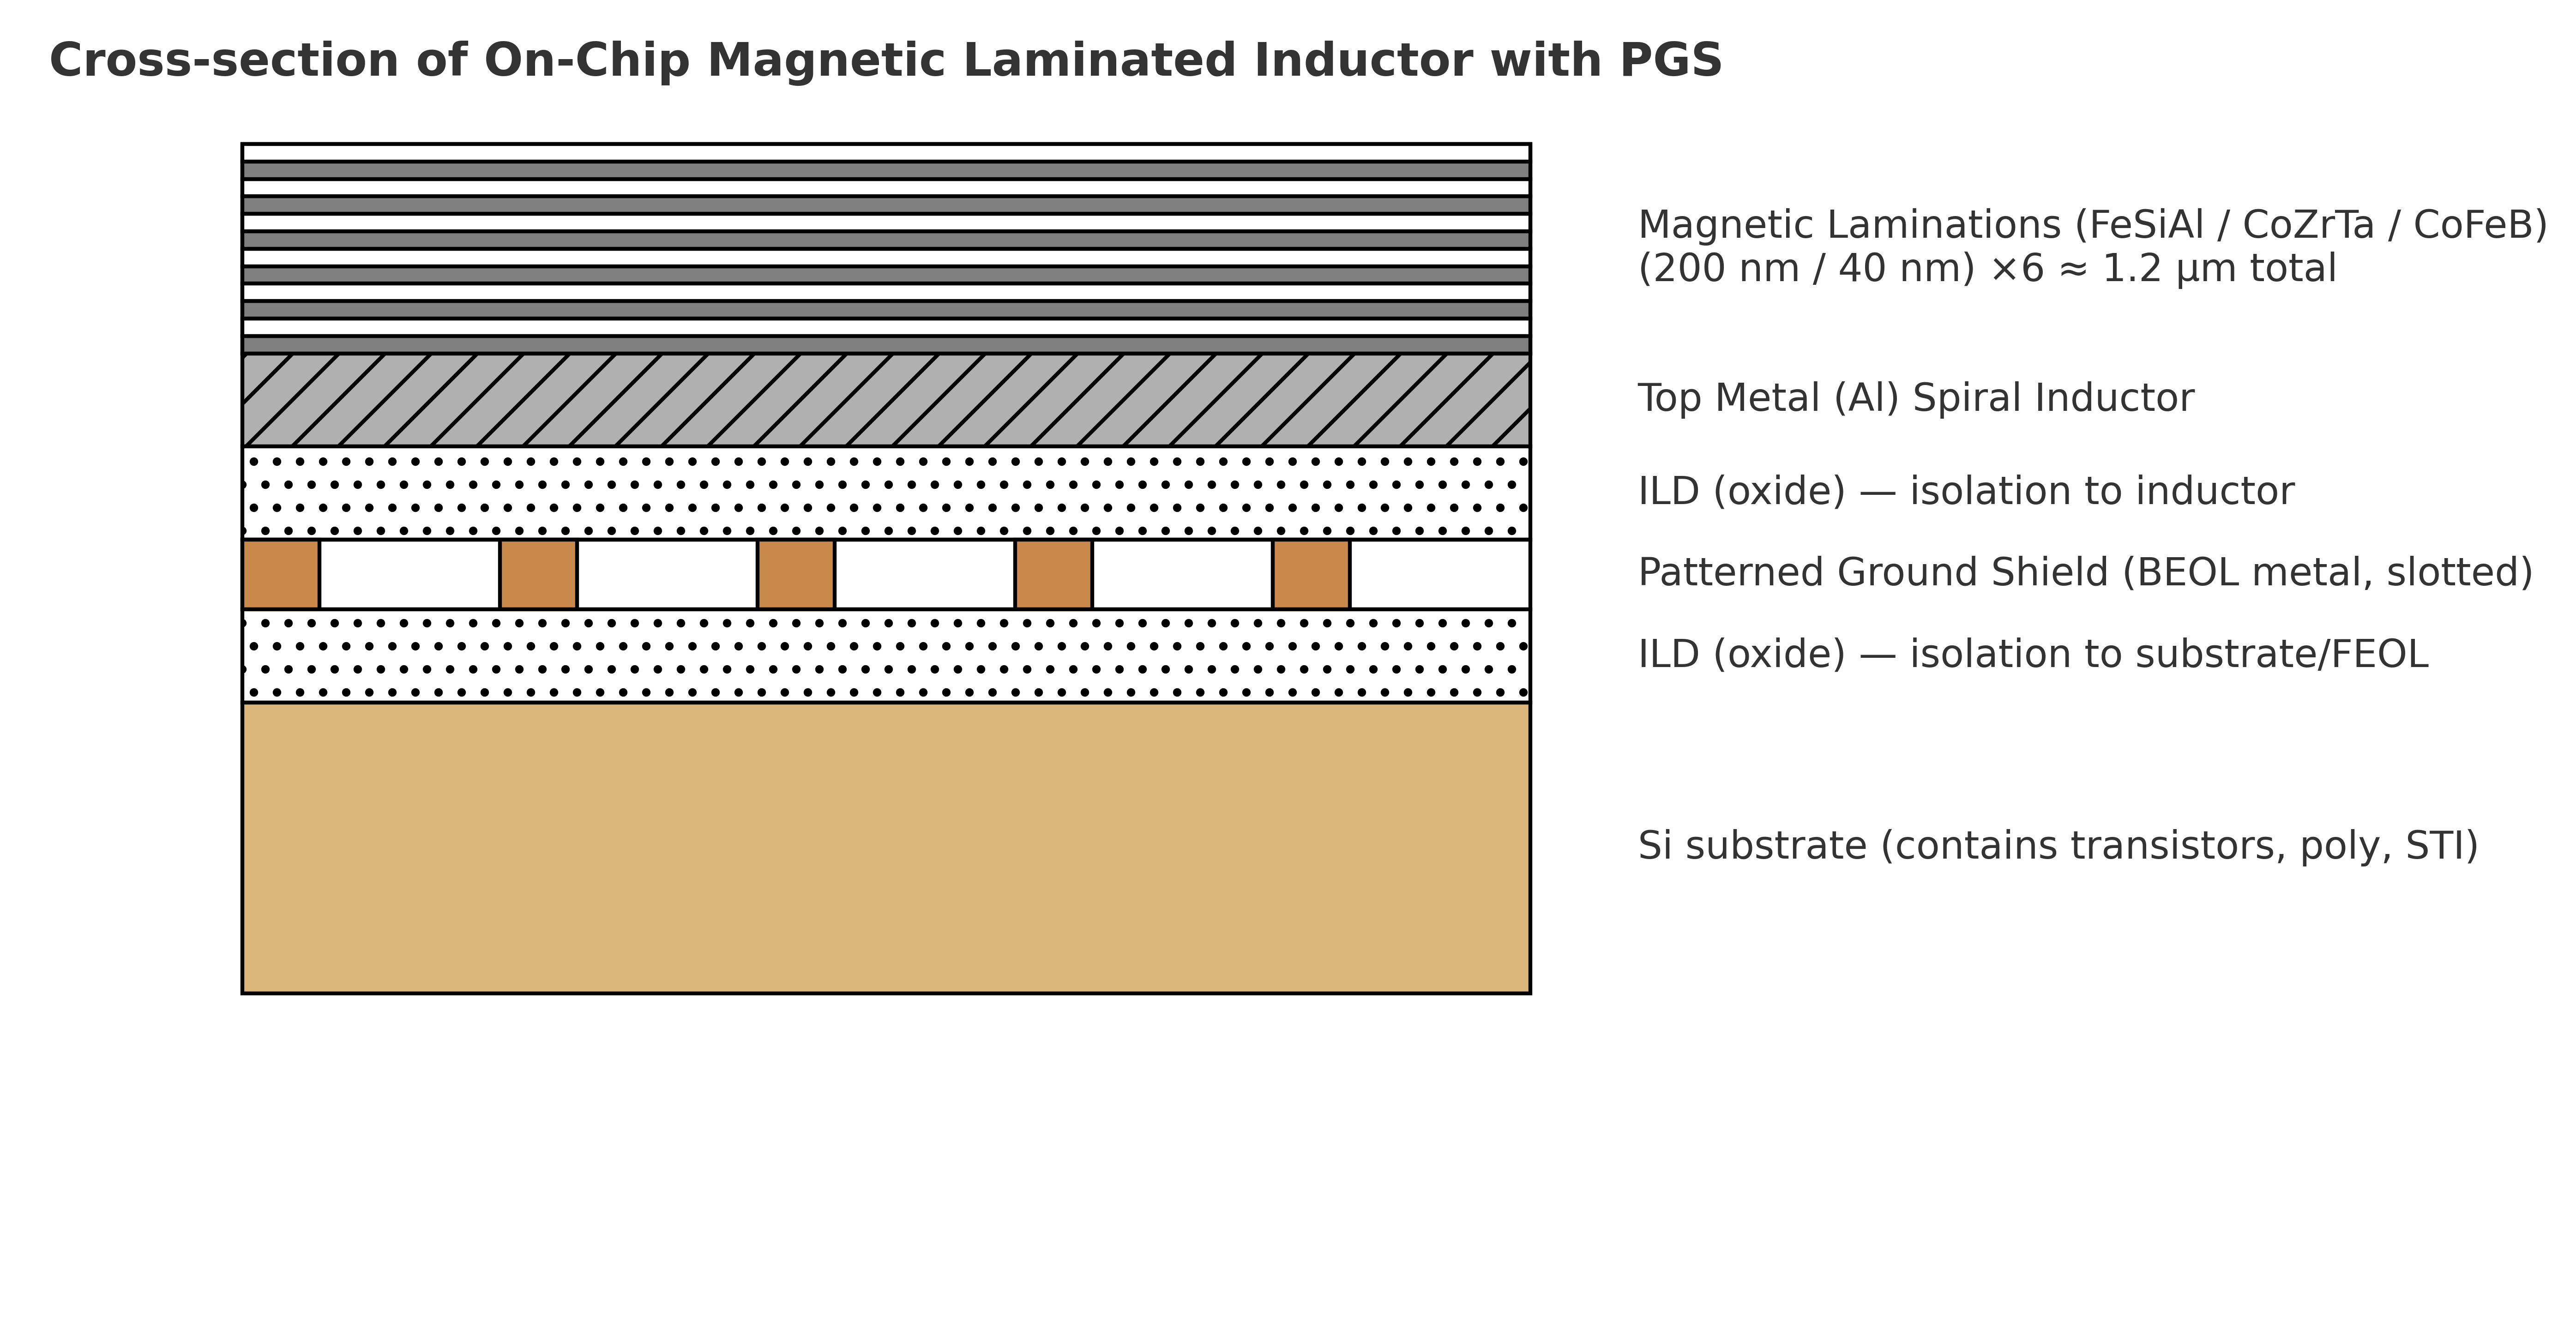
\includegraphics[width=0.9\linewidth]{fig/fig1_laminated_cross_section.png}
\caption{Cross-sectional concept of laminated magnetic inductor with PGS.}
\label{fig1}
\end{figure}

\begin{figure}[!t]
\centering
\begin{tikzpicture}[node distance=2cm,auto,>=latex']
\node[draw, rectangle, minimum width=2.5cm, minimum height=1cm] (buck) {Buck Converter};
\node[draw, rectangle, minimum width=2.5cm, minimum height=1cm, right=of buck] (ldo) {LDO Regulator};
\draw[->, thick] (buck) -- (ldo) node[midway,above]{Clean Supply};
\end{tikzpicture}
\caption{Hybrid Buck-LDO architecture.}
\label{fig2}
\end{figure}

\begin{figure}[!t]
\centering
\begin{tabular}{lcc}
\toprule
Parameter & Air-core & Proposed \\
\midrule
$L$ @ 20 MHz & 40 nH & 100 nH \\
$Q$ @ 20 MHz & 5 & 15 \\
$I_{\mathrm{sat}}$ & 0.2 A & 0.5 A \\
DCR & 0.40 $\Omega$ & 0.20 $\Omega$ \\
Area & 0.8 mm$^2$ & 0.6 mm$^2$ \\
Efficiency & $<65$\% & 80\% \\
Ripple & 5--10 mV & $<1$ mV \\
PSRR @ 1 MHz & 30 dB & $>60$ dB \\
\bottomrule
\end{tabular}
\caption{Performance summary: air-core vs. proposed laminated inductor.}
\label{fig3}
\end{figure}

\end{document}
